% This is "sig-alternate.tex" V2.0 May 2012
% This file should be compiled with V2.5 of "sig-alternate.cls" May 2012
%
% This example file demonstrates the use of the 'sig-alternate.cls'
% V2.5 LaTeX2e document class file. It is for those submitting
% articles to ACM Conference Proceedings WHO DO NOT WISH TO
% STRICTLY ADHERE TO THE SIGS (PUBS-BOARD-ENDORSED) STYLE.
% The 'sig-alternate.cls' file will produce a similar-looking,
% albeit, 'tighter' paper resulting in, invariably, fewer pages.
%
% ----------------------------------------------------------------------------------------------------------------
% This .tex file (and associated .cls V2.5) produces:
%       1) The Permission Statement
%       2) The Conference (location) Info information
%       3) The Copyright Line with ACM data
%       4) NO page numbers
%
% as against the acm_proc_article-sp.cls file which
% DOES NOT produce 1) thru' 3) above.
%
% Using 'sig-alternate.cls' you have control, however, from within
% the source .tex file, over both the CopyrightYear
% (defaulted to 200X) and the ACM Copyright Data
% (defaulted to X-XXXXX-XX-X/XX/XX).
% e.g.
% \CopyrightYear{2007} will cause 2007 to appear in the copyright line.
% \crdata{0-12345-67-8/90/12} will cause 0-12345-67-8/90/12 to appear in the copyright line.
%
% ---------------------------------------------------------------------------------------------------------------
% This .tex source is an example which *does* use
% the .bib file (from which the .bbl file % is produced).
% REMEMBER HOWEVER: After having produced the .bbl file,
% and prior to final submission, you *NEED* to 'insert'
% your .bbl file into your source .tex file so as to provide
% ONE 'self-contained' source file.
%
% ================= IF YOU HAVE QUESTIONS =======================
% Questions regarding the SIGS styles, SIGS policies and
% procedures, Conferences etc. should be sent to
% Adrienne Griscti (griscti@acm.org)
%
% Technical questions _only_ to
% Gerald Murray (murray@hq.acm.org)
% ===============================================================
%
% For tracking purposes - this is V2.0 - May 2012

\documentclass{sig-alternate}

\newenvironment{checklist}{%
  \begin{list}{}{}% whatever you want the list to be
  \let\olditem\item
  \renewcommand\item{\olditem[$\Box$] }
  \newcommand\checkeditem{\olditem[$\CheckedBox$]}

}{%
  \end{list}
}
\newcommand{\ie}{{\em i.e.}}
\newcommand{\eg}{{\em e.g.}}
\newcommand{\ea}{{\em et al. }}

\newcommand\tti[1]{\small\texttt{#1}\normalsize}
\newcommand\ttl[1]{\\* \indent\indent\small\texttt{#1}\normalsize \\*}

\newcommand\system{NetAssay}
%\usepackage{flushend}
\usepackage{fancyvrb}


%\hyphenation{googlevideocontent}

\begin{document}
%
% --- Author Metadata here ---
\conferenceinfo{SIGCOMM}{'14 Chicago, Illinois USA}
%\CopyrightYear{2007} % Allows default copyright year (20XX) to be over-ridden - IF NEED BE.
%\crdata{0-12345-67-8/90/01}  % Allows default copyright data (0-89791-88-6/97/05) to be over-ridden - IF NEED BE.
% --- End of Author Metadata ---

\title{\system{}: Providing New Monitoring Primitives for Network Operators}
%\titlenote{(Produces the permission block, and copyright information). For use with SIG-ALTERNATE.CLS. Supported by ACM.}}
%\subtitle{[Extended Abstract]
%\titlenote{A full version of this paper is available as
%\textit{Author's Guide to Preparing ACM SIG Proceedings Using
%\LaTeX$2_\epsilon$\ and BibTeX} at
%\texttt{www.acm.org/eaddress.htm}}}
%
% You need the command \numberofauthors to handle the 'placement
% and alignment' of the authors beneath the title.
%
% For aesthetic reasons, we recommend 'three authors at a time'
% i.e. three 'name/affiliation blocks' be placed beneath the title.
%
% NOTE: You are NOT restricted in how many 'rows' of
% "name/affiliations" may appear. We just ask that you restrict
% the number of 'columns' to three.
%
% Because of the available 'opening page real-estate'
% we ask you to refrain from putting more than six authors
% (two rows with three columns) beneath the article title.
% More than six makes the first-page appear very cluttered indeed.
%
% Use the \alignauthor commands to handle the names
% and affiliations for an 'aesthetic maximum' of six authors.
% Add names, affiliations, addresses for
% the seventh etc. author(s) as the argument for the
% \additionalauthors command.
% These 'additional authors' will be output/set for you
% without further effort on your part as the last section in
% the body of your article BEFORE References or any Appendices.

\numberofauthors{2} %  in this sample file, there are a *total*
% of EIGHT authors. SIX appear on the 'first-page' (for formatting
% reasons) and the remaining two appear in the \additionalauthors section.
%
\author{
% You can go ahead and credit any number of authors here,
% e.g. one 'row of three' or two rows (consisting of one row of three
% and a second row of one, two or three).
%
% The command \alignauthor (no curly braces needed) should
% precede each author name, affiliation/snail-mail address and
% e-mail address. Additionally, tag each line of
% affiliation/address with \affaddr, and tag the
% e-mail address with \email.
%
% 1st. author
\alignauthor
Sean Donovan\\
       \affaddr{Georgia Institute of Technology}\\
%       \affaddr{1932 Wallamaloo Lane}\\
%       \affaddr{Wallamaloo, New Zealand}\\
       \email{sdonovan@cc.gatech.edu}
% 2nd. author
\alignauthor
Nick Feamster\\
       \affaddr{Georgia Institute of Technology}\\
       \email{feamster@cc.gatech.edu}
}
\maketitle
\begin{abstract}
Home and business network operators have limited network statistics available
over which management decisions can be made. Similarly, there are few triggered
behaviors, such as usage or bandwidths cap for individual users, that are
available. By looking at sources of traffic, based on Domain Name System (DNS)
cues for content of particular web addresses or source Autonomous System (AS) of
the traffic, network operators could create new and interesting rules for
their network. 
\system{} is a Software-Defined Networking (SDN)-based, network-wide monitoring
and reaction framework. By integrating information from Border Gateway Protocol
(BGP) and the Domain Name System, \system{} is able to integrate formerly
disparate sources of control information, and use it to provide better 
monitoring, more useful triggered events, and security benefits for network 
operators.
%Using software-defined networking (SDN), Border Gateway Protocol (BGP) server integration, and parsing Domain Name System (DNS) packets, /system{} is able provide network-wide monitoring at a higher level of abstraction than current, widely used systems. Users are able to look for all traffic coming from \tti{gatech.edu} or look for traffic classified as video, and write rules based off for statistics gathered from these abstractions. 
\end{abstract}

% A category with the (minimum) three required fields
%\category{C.2.3}{Network Operations}{Network management}
%\category{C.2.3}{Network Operations}{Network monitoring}

%\terms{Theory}

\keywords{Network monitoring, network management}

\section{Introduction}
Network management is a complex area. On stub networks, where the network is only a client to other networks, monitoring user behavior is limited. Bandwidth monitoring at the port or address level is among the more complex operations that are available. Similarly, triggered behaviors such as usage caps are limited. 
More complex behavior is available, primarily in highly specialized security appliances, however these are not general purpose devices.

What is needed is a generalized system that can monitor network activity and produce behaviors based on high level policies. For instance, a network operator would like to know how much video traffic each user is consuming in a month, and, if they reach a specified limit, limit their bandwidth for the rest of the month. Right now, there is no easy way of doing this. 

\system{} is being developed to make it easy for network operators to implement such policies. In the video bandwidth example, \system{} needs to decide what network flows are video traffic. Traffic coming from \\\tti{googlevideocontent.com} will be classified as video, as could any traffic associated with AS 2906, Netflix's AS.

More interesting triggered behaviors are also possible. For instance, a network operator has blacklists of ASes and domains that are associated with malicious behavior, but do host some legitimate content that should still be accessible. In this case, if a connection was destined for an IP associated with a potentially malicious AS, the network could automatically redirect traffic to a virus scanning appliance, rather than needing to send all traffic through the appliance. Another use would be to set a limit for amount of data that would be sent to a blacklisted AS before blocking connections, due to suspected bad behavior.

Similar triggered behaviors have been described in prior works~\cite{cloudwatcher}\cite{opensafe}, however this has been limited to network security security devices.

%\subsection{Behavioral Queries}
\section{Example Behaviors}
\label{sec:examples}
Before going into the design, a few examples follow. This is in Pyretic syntax~\cite{pyretic}, where \tti{>}\tti{>} is sequential composition (operations run in order) and \tti{+} is parallel composition (operations run in parallel). 

\begin{Verbatim}[fontsize=\small]
  traffic_in_bytes(to = 'BobsPC', 
                   content = 'video',
                   timespan = 'monthly') > 10**9 >>
      rate_limit(to = 'BobsPC', 
                content = 'video', 
                bandwidth = 65536)
\end{Verbatim}

The example above is a variation on the video bandwidth limitation example. In this case, we only care if Bob's PC is downloading more then 10 gigabytes of video traffic in a month. If it does reach this limit, then we want to limit the bandwidth to 64 kilobytes per second.

\begin{Verbatim}[fontsize=\small]
  match_AS(pkt.srcip, AS = '12345')) >>
      drop()
\end{Verbatim}

The second example is simpler. We are see if a packet came from a AS 12345. If so, we want to drop it. Implicitly, if we do not drop a packet, it will be forwarded.


\section{Design}
%\system{} is an SDN-based system. This provides both a whole-network view of traffic and centralized control, such that all network ingress points are under control of the SDN controller. This allows both of our goals, high-level monitoring and more interesting triggered behaviors, to be possible.

%The system is based on the SDX platform~\cite{sdx}, which provides an easy to use policy syntax. Network operators use the new primitives being created for \system{} as they would if they were creating policies for SDX.

\begin{figure}
    \centering
    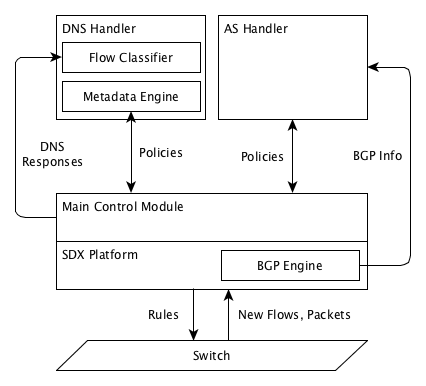
\epsfig{file=./diagrams/architecture, width=.8\columnwidth}
    \caption{\system{} architecture}
    \label{fig:architecture}
\end{figure}


\system{} is SDN-based and works on top of the SDX platform~\cite{sdx}. %This provides easy to understand syntax for network operators.
\system{} is divided into three parts, as can be seen in Figure~\ref{fig:architecture}. There are two monitoring modules, described below, that provide traffic identification and monitoring information to the main control module (MCM). %The MCM is responsible for combining information from the classification modules and, based on the network operator's policies, writing rules into the network switches.%It is a layer on top of the SDX platform.
The MCM is responsible for combining the results from the monitoring modules, and implementing the reactive policies defined by the network operator.

In the examples above, the MCM would be responsible for integrating the resulting policies low level policies from the DNS handler and AS handler for the \tti{traffic\textunderscore{}in\textunderscore{}bytes()} and \tti{match\textunderscore{}AS()} and sending the matched flows or packets to the the \tti{rate\textunderscore{}limit()} and \tti{drop()} actions.

\subsection{DNS Handler}
The DNS handler contains two parts, a flow classifier based on part of FlowQoS~\cite{FlowQoS} and a metadata engine. %The metadata engine requires the flow classifier, but the flow classifier can be used as a standalone module. In fact, the flow classifier is based on a part of FlowQoS~\cite{FlowQoS}, but is entirely rewritten and heavily enhanced.
At startup, the DNS handler creates a rule in all ingress network devices to make a copy of DNS responses, forward one to the actual destination, and forward the second to the DNS handler, and to the flow classifier in particular. The flow classifier parses the DNS packet, extract the domains and associated IPs, and classifies traffic from the IPs based on the domain name. 
For instance, if during the first example in section~\ref{sec:examples} a DNS response from \tti{googlevideocontent.com} with associated IP of 198.51.100.8 was seen, traffic coming from 198.51.100.8 would be assumed to be video until the DNS response time-to-live (TTL) was reached. 

The metadata engine handles policy implementation for DNS-based classification. The metadata engine is responsible for breaking down the high-level policies passed form the MCM into the constituent components, and handling any changes that my occur dynamically (\ie{}, when a new DNS response comes in). It is also responsible for aggregating data, such as aggregating the number of bytes transferred by video sources.

% Continuing with our video example, if a policy is written to calculate how much video traffic is coming into a network, the metadata engine is responsible for breaking down the high-level policy passed from the MCM into the constituent components. That is, for each new IP address associated with the video classification, it is responsible for creating byte-counter rules for each IP, then aggregating the values reported, and returning this information to the MCM.

In the first example in section~\ref{sec:examples}, the new DNS response from \tti{googlevideocontent.com} would cause the metadata engine to create a new byte counter for flows between 198.51.100.8 and Bob's PC. The new counter would be added to the previous policy and added to any prior video byte counter aggregation. The total would be passed up the the MCM to make any decisions based on the total amount of video traffic to Bob's PC.

%The flow classifier has two main components. The first is the DNS-to-classification database. It contains mappings of IP addresses to classifications, along with metadata about the mapping - the DNS lookup string, expiration time, and the time-to-live (TTL) value from the DNS server. The second component is the DNS parser. This performs two actions, making DNS queries (requested by the metadata engine), and parsing all DNS responses, from self-issued requests and from network user requests.

%The metadata engine is the interface to the policies of \system{}. Going back to our video example, when a new DNS entry comes into the flow classifier, and a classification is assigned, the metadata engine looks at it. If it is classified as `video', the metadata engine will push a new rule to create counters per user to the switches.

\subsection{AS Handler}
As \system{} is based on the SDX platform which contains a BGP-engine, we have access to BGP routes. The primary reponsibilities are similar to those of the DNS handler, in that the AS handler needs to break down the high level policy into its consistuent components and returning them to the MCM.
%In the case where a network operator wants to send all traffic from a particular AS to a virus scanner appliance, the AS handler will identify which IP addresses are associated with the specified AS, and return these to the MCM. The MCM can then route the traffic vide the virus scanner appliance.

In the second example from section~\ref{sec:examples}, the AS handler would be responsible for breaking down the \tti{match\textunderscore{}AS()} into the constituent components. These components would be a series \tti{match()} actions on source IP addresses from packets to the IP ranges that AS~12345 was advertising. The parallel composition of all of these \tti{match()} would be composed with the \tti{drop()} action by the MCM.

%the AS Handler will install rules for all traffic originating from that AS's advertised IP address blocks. If the network operator does not trust any traffic that passes through a particular AS, the AS Handler can install rules for any IP address block where the AS is in the AS-Path of the BGP route.

Many networks, in particular home or small business networks, BGP information is not accessible. As such, this handler can be seen as optional.



%%%\subsection{Data Flow}
%Rules are installed at startup of \system{}, so anything that happens subsequently is dynamic. In particular, the DNS and BGP bindings will change, expire, and be repopulated regularly. As such, we will describe a flow for the first example in the previous section.

%At initialization, multiple rules will be created. First, byte count rules for traffic classified as video destined for Bob's PC will be installed. These counts will be reported at a set interval (perhaps once per minute). As category-specific rules are DNS-based, each of the different video counting rules will be summed by the DNS metadata engine and reported to the MCM.

%As Bob visits different video websites, DNS requests will be made by his PC. The responses will be inspected by the DNS flow classifier, while simultaneously forwarding the response to Bob. When Bob does request the video, the source IP will be checked by the DNS metadata module against the DNS database to find out if it has been classified. Since it is a video source, new byte counter rules for the new flow will be installed, and added to the previous rules. 

%Once the 10 gigabyte limit is hit, the MCM will create a \tti{ratelimit} rule and write that to the closest switch to Bob's PC.

%%This section will go into detail of the inner workings of the first example above, about limiting Bob's video consumption. We are only going to discuss the actions of the DNS handler, but the actions of the AS handler will be substantially the same.

%%%Policy is established at startup of \system{}, so anything that happens subsequently is dynamic. In particular, the DNS and BGP bindings will change, expire, and be repopulated regularly. We will now describe part of the behavior of the first example, limiting Bob's video consumption. We are only going to discuss the actions of the DNS handler, but the actions of the AS handler will be substantially the same.

%%%When a new DNS response comes in, the response is parsed and classified. If it is classified as video, the DNS metadata engine will create new rules that establishes byte counters for Bob's PC to all traffic coming from the IP addresses associated with the video site. It does not matter if Bob was associated with the DNS request, the rules would be installed regardless.

%%%There are likely multiple addresses associated with video traffic, and likely as many counters. These counters will need to be accumulated, which is also handled by the DNS metadata engine. The total of the counters is sent to the MCM, which, if the total has reached 10 gigabytes for the month, will create a \tti{ratelimit} rule and write the rule to the closest switch to Bob's PC.


\section{Progress and Future Work}
Work on \system{} is ongoing. Design work is progressing. The DNS flow classifier is complete, though the classification data set is small and video-focused at the moment. 

There are some inherent limitations, but will be resolved thanks to progress on other project. In particular, SDX is limited to a single switch right now, however this may be a minor issue due to ongoing SDX development.

%Of note is that the DNS flow classifier is the only module that does packet inspection.

Future work, beyond finishing currently planned work, is to proactively perform DNS look ups from various public DNS sources in order to get a broader data set. While conflicts between the handlers policies are unlikely, handling conflicts needs to be addressed in the future. Along the same lines, in cases where bandwidth is being counted, preventing `double counting' between the two handlers is also necessary.


%\section{Conclusion}
%\system{} is a work-in-progress for creating a high level monitoring system that provides for better triggered events for network operators. It offers flexability, that most current systems to not, and explores new 
% Most current systems are lacking with the flexibility that is offered to their users, and is an opportunity to make progress on a heretofore unexplored problem.



%
% The following two commands are all you need in the
% initial runs of your .tex file to
% produce the bibliography for the citations in your paper.
\bibliographystyle{abbrv}
\bibliography{sigcomm14poster}  % sigproc.bib is the name of the Bibliography in this case
% You must have a proper ".bib" file
%  and remember to run:
% latex bibtex latex latex
% to resolve all references
%
% ACM needs 'a single self-contained file'!
%

\end{document}
